\documentclass[12 pt,a4paper,twocolumn]{article}
\usepackage[utf8]{inputenc}
\usepackage[T1]{fontenc}
\usepackage[italian,english]{babel}
\usepackage{indentfirst} 
\usepackage{graphicx}
\usepackage{tabularx}
\usepackage{siunitx}
\usepackage{amsmath,stix,bm}
\usepackage{eucal}
\usepackage{caption}

\usepackage{multicol}
\usepackage[includeheadfoot,margin=0.7in,top=0.3 in,bottom=0.35in]{geometry}
%Per grafica vettoriale tramite InkScape%
\usepackage{color}
\usepackage{transparent}
\graphicspath{{img/}}
\usepackage[dvipsnames]{xcolor}
\usepackage{pdfpages}
\usepackage{pgfplots}
\usepackage{textcomp}

\usepackage{xcolor,colortbl}
\usepackage{listings}
\usepackage{cleveref}
\usepackage{caption}
\DeclareCaptionFont{quack}{}
\captionsetup[figure]{font={color=gray,small},labelfont={color=black,sc}}
\captionsetup[table]{font={color=gray,small},labelfont={color=black,sc}}
\captionsetup[subfigure]{font={color=gray,small},labelfont={color=black}}
\addto\captionsenglish{\renewcommand{\figurename}{Fig.}}
\addto\captionsenglish{\renewcommand{\tablename}{Tab.}}
\addto\captionsitalian{\renewcommand{\tablename}{Tab.}}
\crefname{table}{Tab.}{Tabs.}  

\usepackage{cancel}

\usepackage{subcaption}
\usepackage{titlesec}
\titleformat*{\section}{\Large\bfseries\color{myGeneralColor}}
\titleformat*{\subsection}{\large\bfseries\color{myGeneralColor}}
\titleformat*{\subsubsection}{\itshape\bfseries\color{myGeneralColor}}
\definecolor{burntsienna}{rgb}{0.91, 0.45, 0.32}
\definecolor{carrotorange}{rgb}{0.93, 0.57, 0.13}
\definecolor{darktangerine}{rgb}{1.0, 0.66, 0.07}
\definecolor{deepsaffron}{rgb}{1.0, 0.6, 0.2}
\definecolor{flax}{rgb}{0.93, 0.86, 0.51}
\definecolor{lava}{rgb}{0.81, 0.06, 0.13}
\usepackage{pifont}% http://ctan.org/pkg/pifont
\newcommand{\cmark}{\ding{51}}%
\newcommand{\xmark}{\ding{55}}%
\definecolor{mintbg}{rgb}{.63,.79,.95}
\graphicspath{{figures/}{code/figures/}{../code/figures/}} %Setting the graphicspath
\makeatletter
\def\input@path{{figures/}{code/figures/}{../code/figures/}}
\makeatother
\usepackage{import}
\usepackage{authblk}
\pgfplotsset{compat=newest}
\pgfplotsset{plot coordinates/math parser=false}
\newlength\figureheight
\newlength\figurewidth
\usepackage{placeins}
\usepackage{float}
\usepackage{blindtext}
\usepackage{authblk}
\renewcommand\Affilfont{\tiny \color{gray}}

\title{\vspace*{10 pt}\color{myGeneralColor}\Huge\textbf{Simulazione di un modello RLC per la meccanica respiratoria in Simulink}\vspace*{1 pt}}
\author[]{Mastrofini Alessandro}
\affil[]{\small alessandro.mastrofini@alumni.uniroma2.eu}
\renewcommand*{\Authand}{ e }
\date{}
\usepackage{fancyhdr}
\pagestyle{fancy}
\fancyhf{}
	\lhead{\small\color{gray} University of Rome Tor Vergata - MSSF}
\fancyfoot[C]{\small{\thepage\  di \pageref{LastPage}}}
\renewcommand{\headrulewidth}{0pt}

\fancypagestyle{plain}{
	\renewcommand{\headrulewidth}{0pt}
	%\setlength{\headheight}{80 pt} 
	\lhead{\small\color{gray} Modellazione e Simulazione di Sistemi Fisiologici  \\
	Docente: Caselli, Federica \\
	Università degli Studi di Roma Tor Vergata\\
	Ingegneria Medica - 2022}
	\rhead{
\includegraphics[height=45pt]{logo.png} }
	\fancyfoot{}
}
\usepackage{lastpage}
\addtocontents{toc}{\protect\setcounter{tocdepth}{0}}
\usepackage{lipsum}
\usepackage[
backend=bibtex,
style=numeric,
sorting=none
]{biblatex} %Imports biblatex package
\addbibresource{mybib.bib} %Import the bibliography file

\usepackage{listings}
\definecolor{codegreen}{rgb}{0,0.6,0}
\definecolor{codegray}{rgb}{0.5,0.5,0.5}
\definecolor{codestring}{rgb}{0.623, 0.176, 0.588}
\definecolor{backcolour}{rgb}{0.96,0.96,0.96}
\definecolor{bbcolour}{rgb}{0.01,0.03,0.35}
\definecolor{indexcolour}{rgb}{0,0.4,0.4}
\definecolor{myOrange}{rgb}{0.933, 0.313, 0.066}
\definecolor{myBlue}{rgb}{0, 0.298, 0.8}
\lstdefinestyle{mystyle}{
	backgroundcolor=\color{backcolour},   
	commentstyle=\color{codegreen},
	classoffset=1,
	keywordstyle=\color{bbcolour},
	numberstyle=\tiny\color{codegray},
	stringstyle=\color{codestring},
	basicstyle=\ttfamily\small,
	breakatwhitespace=false,  
	breaklines=true,                 
	captionpos=b,                    
	keepspaces=false,                 
	numbers=left,                    
	numbersep=3pt,                  
	showspaces=false,                
	showstringspaces=false,
	showtabs=false,                  
	tabsize=2
}
\lstset{texcl=false, mathescape=true,style=mystyle}
\lstset{emph={%  
		i, j,X%
	},emphstyle={\color{bbcolour}}%
}%
\definecolor{myGeneralColor}{rgb}{0, 0.227, 0.580}
\usepackage{tikz}
\usetikzlibrary{fit}
\usetikzlibrary{shapes.geometric, arrows}
\tikzstyle{startstop} = [rectangle, rounded corners, minimum width=7cm, minimum height=1cm,text centered,  fill=backcolour,text width=6.5 cm,draw=gray]
\tikzstyle{startstop2} = [rectangle, rounded corners, minimum width=5cm, minimum height=2cm,text centered,  fill=backcolour,draw=gray]
\tikzstyle{io} = [trapezium, trapezium left angle=80, trapezium right angle=100, minimum width=7cm, minimum height=1cm, text centered,text width=6.5 cm,  fill=backcolour,draw=gray]
\tikzstyle{io2} = [trapezium, trapezium left angle=70, trapezium right angle=110, minimum width=2cm, minimum height=1cm, text centered,  fill=backcolour,draw=gray]
\tikzstyle{process} = [rectangle, minimum width=7cm, minimum height=1cm, text centered,text width=6.5cm,  fill=backcolour,text badly centered,draw=gray]
\tikzstyle{decision} = [diamond, minimum width=1cm, minimum height=1cm, text centered,  fill=backcolour,draw=gray,text width=2cm]
\tikzstyle{arrow} = [thick,->,>=stealth]
\tikzstyle{process2} = [rectangle, minimum width=3.5cm, text width=3.2cm,minimum height=1cm, text centered, dashed, fill=backcolour,draw=gray]
\tikzstyle{process3} = [rectangle, minimum width=4cm,text width=4cm, minimum height=1cm, text centered,  fill=backcolour,draw=gray]
\tikzstyle{process4} = [rectangle, minimum width=6cm,text width=5.5cm, minimum height=1cm, text centered,  fill=backcolour,draw=gray]

\begin{document}


\twocolumn[{
\begin{@twocolumnfalse} 
		\vspace*{20 pt}
	\begingroup
	\let\center\flushleft
	\maketitle
	\let\endcenter\endflushleft
	\endgroup
	\begin{abstract}
% \noindent
% \noindent\\
% \noindent
% \noindent
% \noindent
\textcolor{blue}{
\lipsum[1]
}

%% ABSTRACT 

	\end{abstract}
	\vspace*{20 pt}
\end{@twocolumnfalse}
}]

\section{Introduzione}

% \noindent
\textcolor{blue}{
	\lipsum[1-2]
}

\section{Background}


SCRIVI QUALCOSA

\subsection{Analogia circuitale}

\begin{figure*}[t!]
	\begin{subfigure}{0.5\linewidth}
		\centering
		\small{
			\def\svgwidth{\linewidth}
			\input{circuit.pdf_tex}}
		\caption{}
		\label{fig:modello}
	\end{subfigure}\hfill
	\begin{subfigure}{0.5\linewidth}
		\centering
		\small{
			\def\svgwidth{0.7\linewidth}
			\input{lung.pdf_tex}}
		\caption{}
	\end{subfigure}\hfill
	\caption{Analogia circuitale della meccanica respiratoria \cite{khoo_physiological_2018} (a); Rappresentazione schematica della divisione del circuito polmonare in due contributi resistivi (vie aeree superiori e inferiori) e in due contributi capacitivi (compliance del polmone e della parete toracica), raffigurate anche la pressione alveolare e pleurica.}
\end{figure*}

Il circuito polmonare può essere analizzando facendo un'analogia con i circuiti elettrici.

In particolare è possibile fare un parallelismo tra il flusso d'aria e la corrente elettrica (flusso di cariche) vedendo e la pressione come la presenza di un potenziale elettrico.
Si rivede allora la resistenza meccanica come il rapporto tra l'incremento di pressione rispetto il flusso, analoga alla resisitenza elettrica. Similmente la compliance non è altro che il rapporto tra l'aumento di volume e l'aumento di pressione, in analogia elettrica è un condensatore.

Il sistema in \cref{fig:modello} è un modello di meccanica respiratoria che trascura la presenza di contributi inerziali (non ci induttanze) e considera la presenza di due compartimenti. Sono separate le vie aeree superiori, con il loro contributo resistivo $R_C$ dalle vie aeree inferiori $R_P$. I due compartimenti sono in serie tra loro ed in serie ai serbatoi d'aria, ovvero le capacità rappresentanti il contributo di compliance della parete $C_W$ e del polmone $C_L$. 
Tali contributi sono in serie proprio perchè il volume d'aria passante è lo stesso. 

A questo si aggiunge anche la capacità di shunt $C_S$ che tiene conto di diversi contributi quali lo spazio morto anatomico, la deformabilità delle vie aeree e la comprimibilità dell'aria. Normalmente questo volume è molto piccolo in condizioni respiratorie normali (in assenza di patologie) e a basse frequenze respiratorie.

Si identificano allora anche le pressioni nei nodi. La pressione alle vie aeree $P_{aw}$, la pressione pleurica $P_{pl}$ e la pressione alveolare $P_A$. Chiaramente l'ingresso del sistema, dato dalla bocca e dalle cavità nasali, è rappresentato dalla pressione all'apertura delle vie aeree $P_{aO}$. 



\subsection{Risposta del sistema}

Il circuito in \cref{fig:modello} può essere descritto dalle seguenti equazioni:

\begin{equation}
	\footnotesize{
	\left\{\begin{array}{l}
		P_{a O}=Q R_{C}+\frac{1}{C_{S}} \int\left(Q-Q_{A}\right) \\
		\frac{1}{C_{s}} \int\left(Q-Q_{A}\right)=Q_{A} R_{P}+\left(\frac{1}{C_{L}}+\frac{1}{C_{W}}\right) \int Q_{A}
	\end{array}\right.}
\label{eq:modello}
\end{equation}

Si ottiene allora la funzione di trasferimento del sistema:

\begin{equation}
		\footnotesize{
\begin{aligned}
	H(s)&=\frac{Q(s)}{P_{a O}(s)}\\
	&=\frac{s^{2}+s \frac{1}{R_{P}}\left(\frac{1}{C_{S}}+\frac{1}{C_{e q}}\right)}{s^{2}\left(R_{C}\right)+s\left(\frac{R_{C}+R_{P}+\frac{R_{C} C_{S}}{C_{e q}}}{C_{S} R_{P}}\right)+\frac{1}{C_{e q} C_{S} R_{P}}}
\end{aligned}}
\label{eq:fdt}
\end{equation}

Dove si esprime la serie delle capacità come ${1\over C_{eq}}={1\over C_{L}}+{1\over C_{W}}$. 


\begin{figure*}[t!]
	\centering
	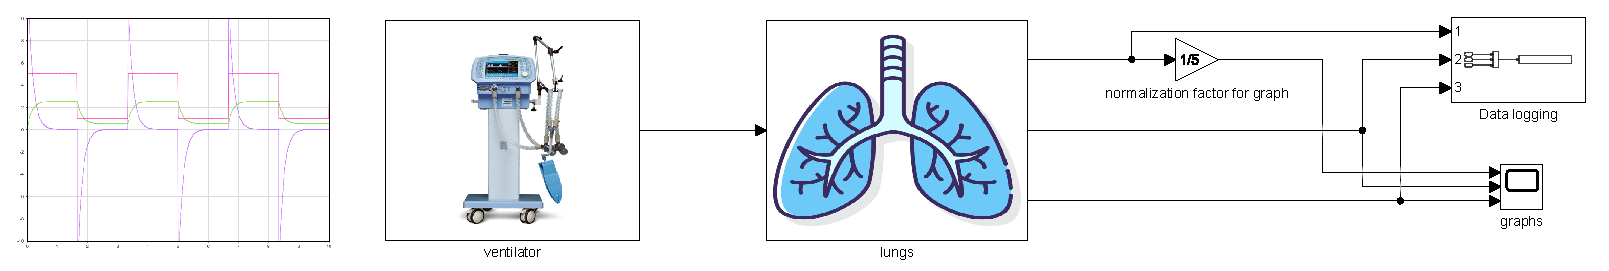
\includegraphics[width=\linewidth]{simulink_base.pdf}
	\caption{Modello del sistema in Simulink diviso in due blocchi principali, uno rappresentante il ventilatore polmonare e l'altro il sistema polmonare, a cui vengono aggiunti un blocco per il salvataggio dei dati e alcune funzioni di visualizzazione.}
	\label{fig:generale}
\end{figure*}

\subsection{Proprietà del sistema}


Chiaramente la soluzione di tale problema richiede la conoscenza della meccanica polmonare propria del paziente. Si assume che il paziente abbia una meccanica polmonare normale.

I coefficienti numerici vengono selezionati da \citeauthor{khoo_physiological_2018} \cite{khoo_physiological_2018}, sono riportati in \cref{tab:coefficienti}.


\begin{table}[h!]
	\centering
	\begin{tabular}{|c|c|c|}
		\hline
		Parametro & Valore & Unità \\ \hline
		$R_C$ & 1 & cm H\textsubscript{2}O s / L \\ \hline
		$R_P$ & 0.5 & cm H\textsubscript{2}O s / L \\ \hline
		$C_L$ & 0.2 & L / cm  H\textsubscript{2}O \\ \hline
		$C_W$ & 0.2 & L / cm  H\textsubscript{2}O \\ \hline
		$C_S$ & 0.005 & L / cm  H\textsubscript{2}O \\ \hline
	\end{tabular}
\caption{Coefficienti numerici per il sistema \cite{khoo_physiological_2018}}
\label{tab:coefficienti}
\end{table}

\subsection{Modellazione del sistema}

La risoluzione del sistema richiede la risoluzione di una ODE e l'approccio, quando le equazioni diventano complesse, è quello di trasferire il modello in un calcolatore. Il classico approccio è di tipo numerico, mediante l'utilizzo di un codice numerico di risoluzioni.

Esiste tuttavia la possibilità di utilizzare Simulink. 

\subsection{Simulink}


Simulink \cite{simulink} è un software sviluppato da MathWorks che fornisce un approccio grafico basato su un ambiente che permette all'utente di convertire il problema in una rete di blocchi di funzioni matematica. 

Inoltre, tale ambiente permette l'integrazione con l'ambiente di Matlab e le relative funzioni di programmazione. 

Un primo approccio sintetico potrebbe essere quello di diagrammare un sistema ingresso-uscita per il tramite della funzione di trasferimento in \cref{eq:fdt}. Tale modello risulterebbe però troppo sintetico e non permetterebbe l'accesso ad alcune variabili esterne, come i singoli flussi.

Si sceglie allora di modellare il sistema completo in \cref{eq:modello}. Tale sistema viene modellato nel blocco \texttt{lungs}. Vengono poi aggiunti anche un sotto sistema per simulare un ventilatore polmonare, ovvero l'ingresso come $P_{aO}$, e un blocco per visualizzare e salvare i dati.

Uno schema generale di alto livello è presente in \cref{fig:generale}


\subsubsection{Sotto sistema del ventilatore}


\begin{figure*}[t!]
	\centering
	\begin{subfigure}{0.4\linewidth}
		\centering
		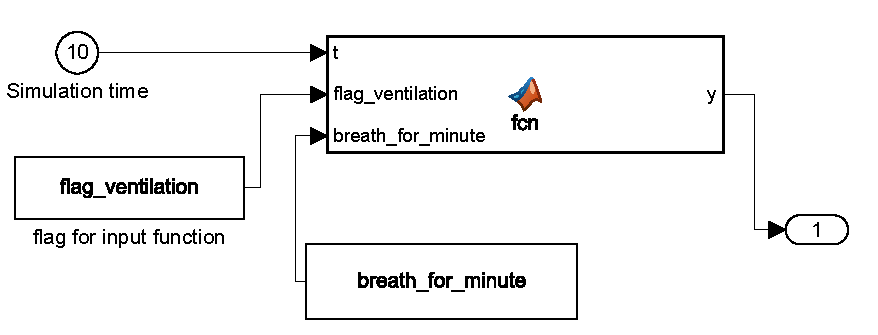
\includegraphics[width=\linewidth]{simulink_ventilator.pdf}
		\caption{}
	\end{subfigure}\hfill
	\begin{subfigure}{0.6\linewidth}
		\centering
		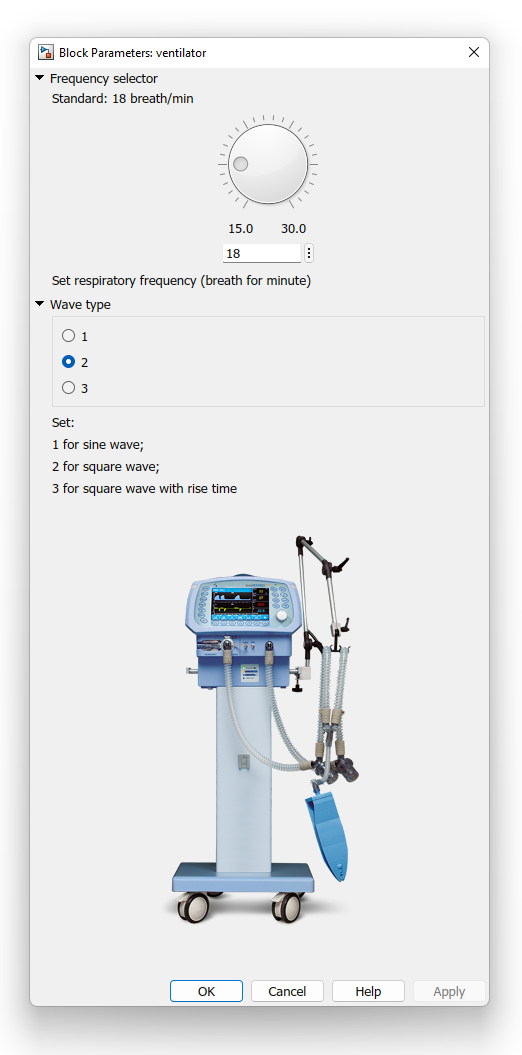
\includegraphics[angle=90,width=0.95\linewidth]{simulink_ventilator_GUI}
		\caption{}
		\label{fig:mask}
	\end{subfigure}\hfill
	\caption{Sistema di input rappresentante il ventilatore: schema a blocchi Simulink dove il segnale di ingresso ($P_{aO}$) viene generato tramite una funzione (\text{fcn}) Matlab (a); GUI tramite la quale è possibile selezionare la frequenza respiratoria e selezionare la forma d'onda.}
\end{figure*}


Nel sotto sistema del ventilatore l'obiettivo è di fornire una $P_{aO}$ con una forma d'onda precisa. Vengono fornite diverse forme d'onda e la frequenza stessa, in atti respiratorio per minuto, può essere variata.

Per fare questo si utilizza un blocco \texttt{funzione Matlab} mediante il quale si può definire un codice Matlab contente la forma d'onda della pressione al variare del tempo di input. Maggiori informazioni sono riportare in appendice. 

Tale blocco richiede anche due variabili ausiliare tramite le quali è possibile scegliere la frequenza respiratoria e il tipo di forma d'onda direttamente dall'interfaccia grafica della maschera del blocco (\cref{fig:mask}). Tramite la maschera di blocco viene anche settata una funzione di callback che permette di aggiornare il nome del file di output, non appena vengono cambiati i parametri, con una struttura del tipo:
\begin{equation*}
	\text{"forma d'onda } + \text{ frequenza } + \text{ .mat"}
\end{equation*}


\subsubsection{Sotto sistema del polmone}


\begin{figure*}[t!]
	\centering
	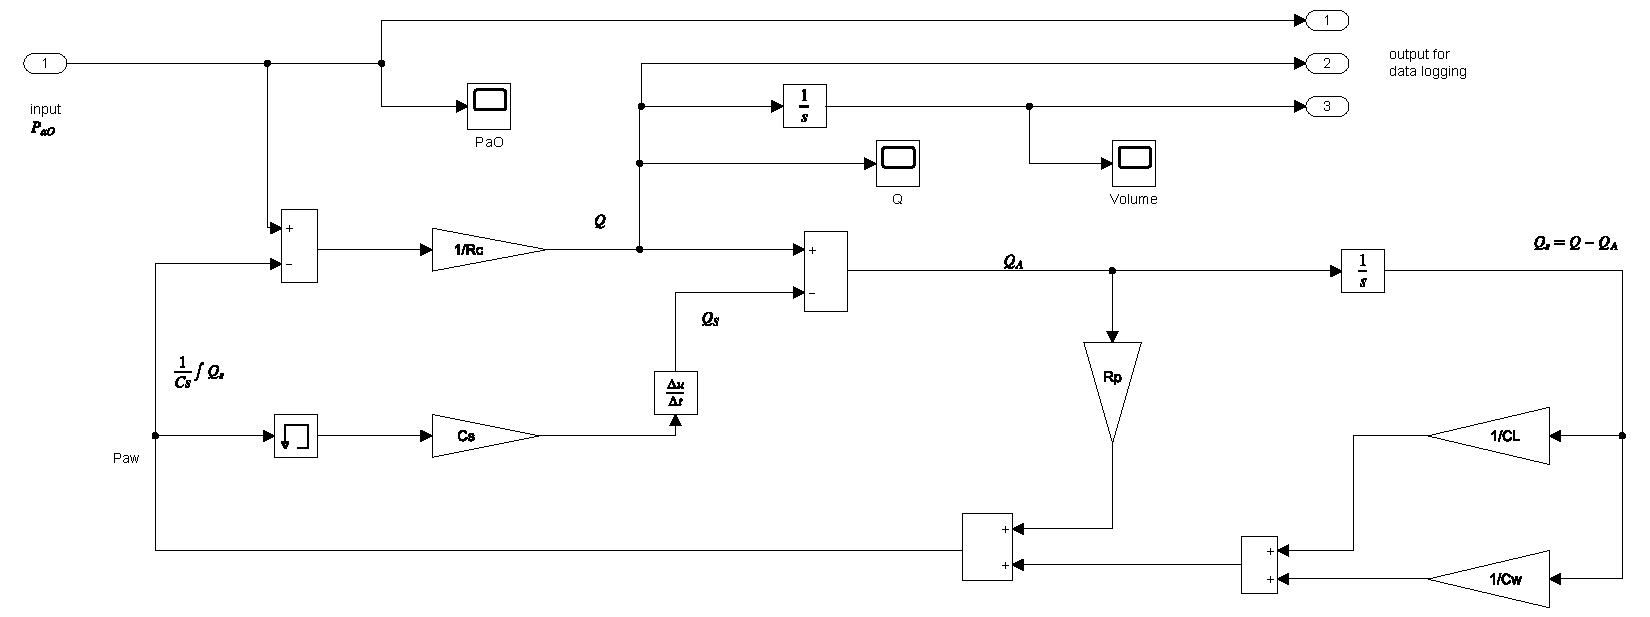
\includegraphics[width=\linewidth]{simulink_lung.pdf}
	\caption{Modello del blocco in Simulink rappresentante il circuito polmonare (in \cref{eq:modello}, \cref{fig:modello})}
	\label{fig:simulinkLung}
\end{figure*}

Le equazioni descrittive del sistema (\cref{eq:modello}) e i relativi segmenti circuitali possono essere rappresentati direttamente nel modello Simulink in \cref{fig:simulinkLung}. 

Tramite la modellazione in Simulink è possibile sommare i contributi di segnale (rappresentanti segmenti del circuito o, equivalentemente, membri dell'equazione), moltiplicare per un costante applicando un guadagno al segnale, derivare e integrare. 
Chiaramente, per passare dal flusso al volume è sufficiente integrare nel tempo. 

Sono presenti anche 3 blocchi di tipo \texttt{scope} per visualizzare le forme d'onda direttamente all'interno della simulazione, il blocco di ingresso (prende il segnale $P_{aO}$ direttamente dal ventilatore) e i 3 blocchi di output utilizzare per salvare i dati. 


\section{Risultati}

\subsection{Ventilazioni ideali}

Un approccio semplice, per analizzare la meccanica polmonare, è quello di ventilare con una forma d'onda ideale. Si utilizza come prima analisi una forma sinusoidale di ampiezza di 2.5 cm H\textsubscript{2}O (ampiezza picco-picco di 5 cm H\textsubscript{2}O) con una frequenza di 15 respiri al minuto \cite{khoo_physiological_2018}. 

\begin{figure*}[t!]
\begin{subfigure}{0.5\linewidth}
	\centering
	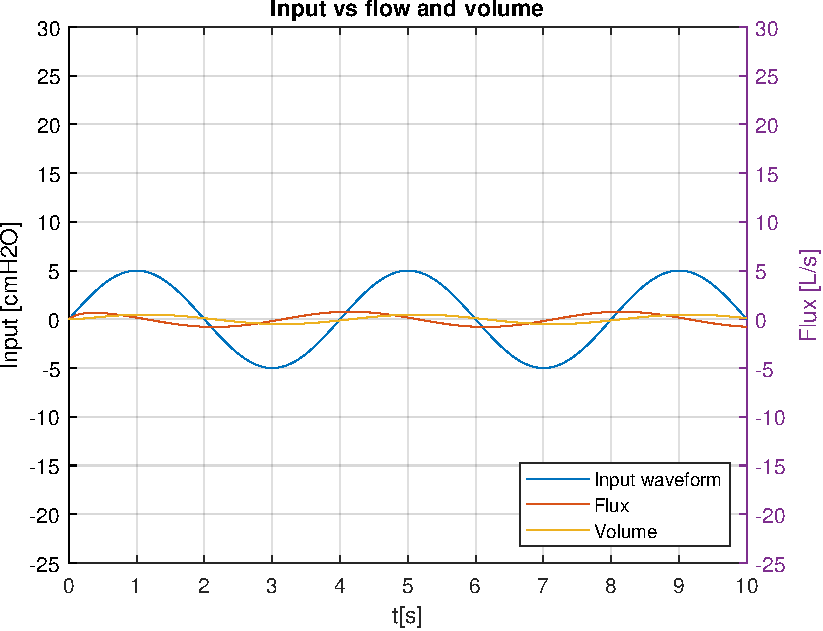
\includegraphics[width=0.95\linewidth]{../model/data_log/data_sine_wave_freq_15.pdf}
	\caption{}
\end{subfigure}\hfill
\begin{subfigure}{0.5\linewidth}
	\centering
	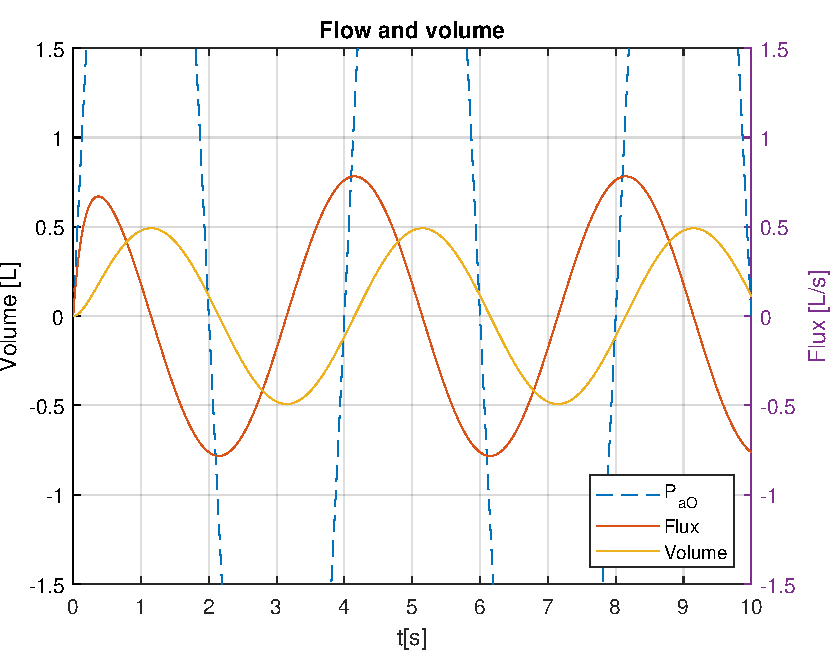
\includegraphics[width=0.95\linewidth]{../model/data_log/data_sine_wave_freq_15_zoom.pdf}
	\caption{}
\end{subfigure}
\caption{Confronto tra la pressione in ingresso con forma d'onda sinusoidale ideale con l'andamento del flusso e del volume (a); ingrandimento sull'andamento di flusso e volume (b). Si può osservare come volume e sfasamento presentano uno sfasamento di 90°. Inoltre, ne flusso ne volume sono in fase con l'andamento della $P_{aO}$. }
\label{fig:sine_wave_15}
\end{figure*}

% This demonstrates that lung mechanics is dominated by compliance effects at such low frequencies. The peak-to-peak change in volume (i.e., tidal volume) is approxi­ mately 0.5 L, while peak Q is ∼0.4 L s  increases (to ∼1.2 L s-1) while tidal volume is decreased (to ∼0.4 L). Now, Q has become more in phase with Pao while volume displays a significant lag. Thus, resistive effects have become more dominant at the higher frequency. The changes in peak Q and tidal volume with frequency demonstrate the phenomenon pulmo­ nologists refer to as frequency dependence of pulmonary resistance and compli­ ance, that is, the lungs appear stiffer and less resistive as frequency increases from resting breathing. 

\textcolor{blue}{
	\lipsum[1-4]
}
\section{Conclusioni}

\textcolor{blue}{
	\lipsum[1-2]
}
%\pagebreak
\section*{Disponibilità dei dati}

Il materiale è disponibile alla repository online del progetto: \url{https://github.com/mastroalex/resp-mech-simulink}

\subsection*{Codice}

\raggedbottom

\pagebreak
\printbibliography[title=Riferimenti]
%\section*{References}


\clearpage
\section*{Appendice}

\subsection*{Codice per la generazione della pressione di ingresso}


\end{document}